% *******************************************************************************
% * Copyright (c) 2007 by Elexis
% * All rights reserved. This document and the accompanying materials
% * are made available under the terms of the Eclipse Public License v1.0
% * which accompanies this distribution, and is available at
% * http://www.eclipse.org/legal/epl-v10.html
% *
% *  $Id: trustx.tex 2933 2007-07-29 10:05:35Z rgw_ch $
% *******************************************************************************
% !Mode:: "TeX:UTF-8" (encoding info for WinEdt)

\section{Elexis-TrustX-Embed }
\label{trustx}
Avec ce plugin les factures du médecin peuvent directement être transmises à un centre de confiance qui échangent des données selon le standard TrustX. (la majorité des centres de confiances en Suisse  fonctionnent avec ce standard) Ce Plugin fonctionne actuellement seulement sous Windows. 

Ce plugin est un peu hors de la ligne du concept de Elexis car il est de multiples manières dépendant des logiciels qui travaillent en mode ClosedSource, raison pour laquelle il ne fonctionne pas sur tous les systèmes d'exploitation comme Elexis. Malheureusement il est actuellement impossible d'éviter ces dépendances car le système TrustX lui-même est basé sur des sources tenues secrètes et puisqu'il prend recours à l'ASAS qui est de son côté aussi une variante ClosedSource d'un public-key-tunnel.
Si vous souhaitez en tant que client du centre de confiance et de ASAS que cette situation change, veuillez demander pour une implémentation OpenSource des interfaces pour le transfer des données. (En effet il n'y a aucune raison objective contre cette demande. Un bon cryptage n'est jamais basé sur la tenue secrète des sources mais sur la forec de l'algorithme.)
Après cette introduction maintenant aux conditions mentionnées. 

\subsection{Conditions}
Vous avez besoin d'Elexis installé sur un ordinateurs avec système d'exploitation Windows. Elexis doit contenir le plugin elexis-tarif des médecins-Suisse (chose qui est toujours le cas car inclus d'emblée). En plus il vous faut d'un \href{http://www.hin.ch}{HIN-Account} et d'un \href{http://www.hin.ch/asas}{ASAS-Client}. En fin de compte aussi le  \href{http://www.trustx.ch/trustx-praxis/documents/setup-2_1_14.exe}{TrustX-Client} doit être installé. Le ASAS-Client de même que le TrustX-Client doit être  configuré correctement.

\subsection{Installation}
Il suffit de télécharger le \href{http://www.elexis.ch/files/elexis-trustx-embed.zip}{elexis-trustx-embed- Plugin} et de le décompresser dans le registre d'Elexis. Le plugin sera à disposition après le prochain démarrage d'Elexis.

\subsection{mode de fonctionnement}
\begin{wrapfigure}{l}{6cm}
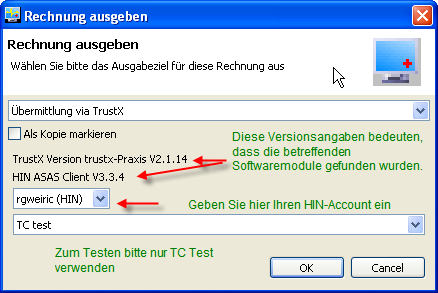
\includegraphics[width=6cm]{images/trustx.png}
\caption{TrustX-Transfer}
\label{fig:trustx}
\end{wrapfigure}
% trustx.png: 438x293 pixel, 96dpi, 11.59x7.75 cm, bb=0 0 328 220

Trustx-embed se branche sur le système d'édition de la facturation. Lorsque vous faites une facture vous pouvez utiliser au lieu de l'imprimante l'option \textit{Transmission via Trustx} ce qui fait apparaître le dialogue suivant la Fig. \ref{fig:trustx}:

Assurez-vous que TrustX et ASAS avaient été trouvés correctement et choisissez le bon Account et le bon centre de confiance. Après un clic toutes les factures seront d'abord sauvegardées par le tunnel ASAS et ensuite envoyées au centre de confinance.

\subsection{rejets}
Surtout au début il vous arrivera à plusieurs reprises que des fatures sont rejetées par le centre de confiance. De temps en temps le garant manque ou le code EAN du répondant des coûts manque etc. tous des problèmes qui n'avaient pas autant d'importance lors de la facturation sur papier. Toutes les factures rejetées auront le statut \textit{eronné} et peuvent par ceci être retrouvées et corrigées dans la View 'factures'.

Avant d'envoyer les factures veuillez être attentifs aux points suivants :
\begin{itemize}
 \item Toute facture doit être attribuée à un cas qui a
\begin{itemize}
 \item un garant et un répondant des coûts
\item et un mandant.
\end{itemize}
\item Toute facture doit contenir au moins un diagnostic ou un code de diagnostic. Ceci est le car lorsque vous avecz introduit dans au moins une des consultations facturées un diagnostic. (Ceci vaut pour TrustX)
\item Le mandant doit avoir un code EAN correcte (qui doit être introduit par ex. dans la perspective \textit{contacts}). Vous pouvez demander à la FMH quel est votre code EAN si jamais il ne vous est pas encore connu.
\item Le répondant des coûts doit aussi avoir un code EAN correcte (qui doit être introduit par ex. dans la persepective \textit{contacts}). Vous pouvez demander les codes EAN directement chez les assureurs ou vous pouvez consulter une des listes qui sont accessibles sur internet comme par ex. sur le site \href{http://www.sgim.ch/info/tarmed/EAN_KV.pdf}{SGIM}.

\end{itemize}

\textit{Le développement de ce plugin a été financé par le Docteur S. Henzi Bern qui le met gratuitement à disposition à tous les utilisateurs de Elexis.}


